\chapter{Pipeline extraction} \label{chapter5}
\minitoc
\eject

% The previous chapter presented globally the state of the art in designing systems to scale in performance, and in maintenance.
% It refined the scope of this thesis to the study of the opposition between maintenance scalability and performance scalability in streaming web applications.
% It concluded with the objectives of this thesis, which is to find an equivalence between the two opposed organizations.
% The maintenance scalability organization, supported by modular programming, higher-order programming and a global memory store.
% The performance scalability organization, supported by the parallelism of memory and execution distribution.
This chapter presents the first step in the transformation from the event-driven execution model to the pipeline architecture, as presented in figure \ref{fig:roadmap}.
That is to identify and extract a pipeline of execution inside an application following the event-driven execution model.
% In this work, we focus on Javascript, and specifically on \textit{Node.js} applications.
%
% Javascript allows higher-order programming.
% It allows to manipulate functions like any object.
% For example to link them to react to asynchronous events, \textit{e.g.} user inputs and remote requests.
% These asynchronously triggered functions are named callbacks, and allow to efficiently cope with the distributed and inherently asynchronous architecture of the Internet.
% To execute a suite of asynchronous functions, callbacks are nested one into the other.
% This nesting, if not organized properly, can result in unreadable layer of callbacks, commonly presented as \textit{callback hell}\ftnt{http://maxogden.github.io/callback-hell/}, or \textit{pyramid of doom}.
%
% Promises are another way to organize a suite of asynchronous operations avoiding this callback hell.
% They organize the operations as a well-defined pipeline.
% Moreover, Promises provide additional control over the asynchronous execution flow, than callbacks.
% They are part of the next version of the Javascript language, ECMAScript 6\ftnt{http://people.mozilla.org/~jorendorff/es6-draft.html}.
% To avoid the equivalence being unnecessarily incomplete, we present an alternative to Promise, called Due.
% Due organize the operations like Promises, as a well-defined pipeline, while discarding the unnecessary additional control over the asynchronous flow.
%

This chapter focus on the identification of the chains of causality in continuations.
Promises bring more control over the asynchronous flow than the chaining of causal sequentiality.
But they force another control over the execution flow.
According to the outcome of the operation, they call one function to continue the execution with the result, or another to handle errors.
This conditional execution is indivisible from the Promise structure.
As a result, Promises impose a convention on how to hand back the outcome of the deferred computation, while classic continuations leave this conditional execution to the developer.
To rule out this differences between continuations and Promises, section \ref{chapter5:dues} introduces a simpler specification to Promise, called Due.

This chapter presents a compiler to identify the pipeline of operating underlying in a Javascript application. % using callbacks, and extract it to express it as Dues.
The compiler expresses this pipeline as chains of Dues.

Section \ref{chapter5:equivalence} explains the transformation from imbrications of continuations to sequences of Dues.
Section \ref{chapter5:compiler} presents a compiler to automate the application of this equivalence.
And finally, the developed compiler is evaluated in section \ref{chapter5:evaluation}.
This compiler has been tested over 64 \textit{Node.js} packages from the node package manager (npm\ftnt{https://www.npmjs.com/}).
55 packages were incompatible with the compiler, 9 packages were compiled with success.


% \subsection{From continuations to Promises} \label{seciton:definitions:analysis}

% As detailed in the previous sections, continuations provide the control over the sequentiality of the asynchronous execution flow.
% Promises improve this control to allow chained compositions, and unify the syntax for the synchronous and asynchronous paradigm.
% This chained composition brings a greater clarity and expressiveness to source codes.
% At the light of these insights, it makes sense for a developer to switch from continuations to Promises.
% However, the refactoring of existing code bases might be an operation impossible to carry manually within reasonable time.
% We want to automatically transform an imbrication of continuations into a chained composition of Promises.

% We identify two steps in this transformation.
% The first is to provide an equivalence between a continuation and a Promise.
% The second is the composition of this equivalence.
% Both steps are required to transform imbrications of continuations into chains of Promises.
% to be able to compose this equivalence for imbrications of continuations to obtain chains of Promises.

% Because Promises bring chained composition, the first step might seem trivial as it does not imply any imbrication to transform into chain.
% However, as explained in section \ref{section:definitions:promise}, Promises impose a control over the execution flow that continuations leave free.
% This control induces a common convention to hand back the outcome to the continuation.

% In the Javascript landscape, there is no dominant convention for handing back outcomes to continuations.
% In the browser, many conventions coexist.
% For example, \textit{jQuery}'s \texttt{ajax}\ftnt{http://api.jquery.com/jquery.ajax/} method expects an object with different continuations for success, errors and various other events during the asynchronous operation.
% \textit{Q}\ftnt{http://documentup.com/kriskowal/q/}, a popular library to control the asynchronous flow, exposes two methods to define continuations: \texttt{then} for successes, and \texttt{catch} for errors.
% % The conventions for continuations are very heterogeneous in the browser.
% On the other hand, the \textit{Node.js} API always used the \textit{error-first} convention, encouraging developers to provide libraries using the same convention.
% In this large ecosystem the \textit{error-first} convention is predominant.
% All these examples use different conventions than the Promise specification detailed in section \ref{section:definitions:promise}.
% They present strong semantic differences, despite small syntactic differences.
% % Some conventions include the conditional execution over the outcome, while other conventions let developers provide it.
% % These conventions uses different control-flow.

% To translate these different conventions into the Promises one, the compiler would need to identify them.
% Such an identification might be possible with static analysis methods such as the points-to analysis~\cite{Wei2014}, or a program logic~\cite{Gardner2013,Bodin2014}.
% However, it seems impracticable because of the number and semantical heterogeneity of these conventions.
% Indeed, in the browser, each library seems to provide its own convention.

% In this paper, we are interested in the transformation from imbrications to chains, not from one convention to another.
% The \textit{error-first} convention, used in \textit{Node.js}, is likely to represent a large, coherent code base to test the equivalence.
% Indeed contains currently more than 125 000 packages.
% For this reason, we focus only on the \textit{error-first} convention.
% Thus, our compiler is only able to compile code that follows this convention.
% The convention used by Promises is incompatible.
% We propose an alternative specification to Promise following the \textit{error-first} convention.
% In the next section we present this specification called Due.

% The choice to focus on \textit{Node.js} is also motivated by our intention to compare later the chained sequentiality of Promises with the data-flow paradigm.
% \textit{Node.js} allows to manipulate streams of messages.
% This proved to be efficient for real-time web applications manipulating streams of user requests.
% Both Promises and data-flow arrange the computation in chains of independent operations.
% % In section \ref{section:equivalence}, we explain the two steps of the transformation from continuations to Dues.









% Dues are further defined in section \ref{section:definitions}.


% This made Javascript a language of choice to develop both client and, more recently, server applications for the web.

% Callbacks are well-suited for small interactive scripts.
% But in a complete application, they are ill-suited to control the larger asynchronous execution flow.
% Their use leads to intricate imbrications of function calls and callbacks, commonly presented as \textit{callback hell}\ftnt{http://maxogden.github.io/callback-hell/}, or \textit{pyramid of doom}.
% This is widely recognized as a bad practice and reflects the unsuitability of callbacks in complete applications.
% Eventually, developers enhanced callbacks to meet their needs with the concept of Promise~\cite{Liskov1988}.

% Promises bring a different way to control the asynchronous execution flow, better suited for large applications.
% They fulfill this task well enough to be part of the next version of the Javascript language, ECMAScript 6\ftnt{http://people.mozilla.org/~jorendorff/es6-draft.html}.
% However, because Javascript started as a scripting language, beginners are often not introduced to Promises early enough.
% Most APIs use the classical callback approach encouraging beginner in this practice.
% Moreover, despite its benefits, the concept of Promise is not yet widely acknowledged.
% Developers may implement their own library for asynchronous flow control before discovering existing ones.
% There is such a disparity between the needs for and the adoption of Promises libraries, that there are almost 40 different implementations\ftnt{https://github.com/promises-aplus/promises-spec/blob/master/implementations.md}.

% With the upcoming introduction of Promise as a language feature, we expect an increase of interest, and believe that many developers will shift to this better practice.
% In this paper, we propose a compiler to automate this shift in existing code bases.
% We present the transformation from an imbrication of callbacks to a sequence of Promise operations, while preserving the semantic.

% Promises bring a better way to control the asynchronous execution flow, but they also impose a conditional control over the result of the execution.
% Callbacks, on the other hand, leave this conditional control to the developer.
% This paper focuses on the transformation from imbrication of callbacks to chain of Promises.
% To avoid unnecessary modifications on this conditional control, we introduce an alternative to Promises leaving this conditional control to the developer, like callbacks.
% We call this simpler specification Dues.
% Our approach enables us to compile legacy Javascript code and brings a first automated step toward full Promises integration.
% This simple and pragmatic compiler has been tested over 64 \textit{Node.js} packages from the node package manager (npm\ftnt{https://www.npmjs.com/}), 9 of them with success.

% In section \ref{section:definitions} we define callbacks, Promises and Dues.
% In section \ref{section:equivalence}, we explain the transformation from imbrications of callbacks to sequences of Dues.
% In section \ref{section:compiler}, we present a compiler to automate the application of this equivalence.
% In section \ref{section:evaluation}, we evaluate the developed compiler.

\section{Dues} \label{chapter5:dues}

% \subsection{Due} \label{section:definitions:due}

A Due is an object used as placeholder for the eventual outcome of a deferred operation.
% Dues are a simplification of the Promise specification.
They are essentially similar to ECMAScript Promises\ftnt{http://www.ecma-international.org/ecma-262/6.0/\#sec-promise-objects}, except for the convention to hand back outcomes.
% They leave the control over the conditional execution over the outcome to the developer.
They use the \textit{error-first} convention, like \textit{Node.js}, as illustrated line \ref{lst:due:error-first} in listing \ref{lst:due}.
The implementation of Dues and its tests are available online\ftnt{https://www.npmjs.com/package/due}.
A more in-depth description of Dues and their creation follows in the next paragraphs.
% The \texttt{mock} method is implemented in listing \ref{lst:due-creation}.
% While a promise expects two continuations, \texttt{onSuccess} and \texttt{onErrors}, the method \texttt{then} of a due expects only one continuation, following the convention \textit{error-first}.
% \footnotemark{\ref{ftn:error-conventions}}
% \footnotemark{\ref{ftn:error-first}}.

\begin{code}[js, %
             caption={Example of a due}, %
             label={lst:due}] %
var my_fn_due = require('due').mock(my_fn); //@\label{lst:due:mock}@

var due = my_fn_due(input);

due.then(function continuation(error, result) { //@\label{lst:due:error-first}@
  if (!error) {
    console.log(result);
  } else {
    throw error;
  }
});
\end{code}

A due is typically created inside the function which returns it.
In listing \ref{lst:due}, line \ref{lst:due:mock}, the \texttt{mock} method wraps the original function \texttt{my\_fn} in a Due-compatible function \texttt{mocked\_fn}.
The rest of this code is similar to the Promise example, listing \ref{lst:then}.

We illustrate in listing \ref{lst:due-creation} the creation of a Due.
The \texttt{mock} method, defined line \ref{lst:due-creation:new}, returns a Due compatible function.
That is a function that returns a Due, instead of expecting a continuation.

At its creation, line \ref{lst:due-creation:new}, the Due expects the original function as argument, which is \texttt{my\_fn} here.
The original function is executed immediatly at the call of the Due-compatible function \textit{mocked\_fn}.
The \texttt{settle} function passed as argument, line \ref{lst:due-creation:new}, is used as a continuation for the original function to settle the Due. %, synchronously or asynchronously.
Therefore, the \texttt{settle} function is pushed at the end of the list of arguments, line \ref{lst:due-creation:push}.
% Indeed, the operation might be synchronous, or asynchronous.
The callback invokes the deferred operation with this list of arguments, and the current context, line \ref{lst:due-creation:call}.
% \texttt{my\_fn} being asynchronous, it expects a callback as last argument : \texttt{settle}.
When finished, the latter calls \texttt{settle} to settle the Due and save the outcome.
% A Due is in one of two mutually exclusive states: settled or pending.
The created Due is returned synchronously.
Its \texttt{then} method allows to define a continuation to retrieve the saved outcome, and continue the execution after its settlement.
If the deferred operation is synchronous, the Due settles during its creation and the \texttt{then} method immediately calls this continuation.
If the deferred operation is asynchronous, this continuation is called during the Due settlement.

% This continuation is defined by the \texttt{then} method.
% After the settlement of the Due, its continuation is executed with the outcome.
% Dues expose a \texttt{then} method expecting a continuation to continue the execution after its settlement.

\begin{code}[js, %
             caption={Creation of a due}, %
             label={lst:due-creation}] %
Due.mock = function(my_fn) { //@\label{lst:due-creation:mock}@
  return function mocked_fn() { //@\label{lst:due-creation:mocked}@
    var _args = Array.prototype.slice.call(arguments),
        _this = this;

    return new Due(function(settle) {  //@\label{lst:due-creation:new}@
      _args.push(settle);  //@\label{lst:due-creation:push}@
      my_fn.apply(_this, _args); //@\label{lst:due-creation:call}@
    })
  }
}
\end{code}

The composition of Dues is the same than for Promises, as illsutrated in listing \ref{lst:dues-sequence}.% explained in section \ref{chapter4:event-loop:promise}.
% This composition is explained in details in section \ref{section:definitions:promise}. %, and illustrated specifically for Dues in listing \ref{lst:dues-sequence}.
Through this chained composition, Dues arrange the execution flow as a sequence of actions to carry on inputs.

\begin{code}[js, %
             caption={Dues are chained like Promises}, %
             label={lst:dues-sequence}] %
var Due = require('due');

var my_fn_due_1 = Due.mock(my_fn_1),
    my_fn_due_2 = Due.mock(my_fn_2),
    my_fn_due_3 = Due.mock(my_fn_3);

my_fn_1(input)
.then(my_fn_2)
.then(my_fn_3)
.then(console.log);
\end{code}

This simplified specification adopts the same convention than \textit{Node.js} for continuations to hand back outcomes.
Therefore, the equivalence between a continuation and a Due is trivial.
% This equivalence, and its composition are explained in details in section \ref{section:equivalence}.
Dues are admittedly tailored for this work, hence, they are not designed to be written by developers, like Promises are.
They are an intermediary step between classical continuations and the second step of the transformation, presented in chapter \ref{chapter6}.
The next section presents the equivalence between continuations and Dues.


% In listing \ref{lst:due}, \texttt{due} is settled when the function \texttt{settle} is called.
% If \texttt{due} is settled, a call to \texttt{due.then(onSettlement)} immediately call the function \texttt{onSettlement}.
% A due is pending if it is not settled.
% A due is resolved if it is settled or if it has been linked with another due.
% Attempting to settle a resolved due has no effect.
% A resolved due may be pending or settled, while an unresolved due is always in the pending state.
% The \texttt{Due} object only exposes the \texttt{then} method.
% \textbf{\texttt{Due.prototype.then(onSettlement)}}\\
% Appends settlement handlers to the due, and returns a new due resolving to the return value of the called handler.
% If the value is a \textit{thenable}, \textit{i.e.} has a method \texttt{then}, the returned due will follow that \textit{thenable}, adopting its eventual state; otherwise the returned due will be fulfilled with the value.
% We present in appendix \ref{section:dueimpl} a simple implementation of Due in Javascript.

\section{From Continuations to Dues} \label{chapter5:equivalence}

This section presents the transformation from a nested imbrication of continuations into a chain of Dues.
It explains the three limitations imposed by the compiler for this transformation to preserve the semantic.
They preserve the execution order, the execution linearity and the scopes of the variables used in the operations.

\subsection{Execution order}

The compiler spots function calls with a continuation, which are similar to the abstraction in (\ref{eq:order:source}).
It wraps the function $fn$ into the function $fn_\textbf{due}$ to return a Due.
And it relocates the continuation in a call to the method $\textbf{then}$, which references the Due previously returned.
The result should be similar to (\ref{eq:order:target}).
The differences are highlighted in bold font.
\begin{equation} \label{eq:order:source}
fn([arguments], continuation)
\end{equation}
\begin{equation} \label{eq:order:target}
fn_\textbf{due}([arguments])\textbf{.then}(continuation)
\end{equation}

The execution order is different whether $continuation$ is called synchronously, or asynchronously.
If $fn$ is synchronous, it calls the $continuation$ within its execution.
It might execute $statements$ after executing $continuation$, before returning.
If $fn$ is asynchronous, the continuation is called after the end of the current execution, after $fn$.
The transformation erases this difference in the execution order.
In both cases, the transformation relocates the execution of $continuation$ after the execution of $fn$.
For synchronous $fn$, the execution order changes ; the execution of $statements$ at the end of $fn$ and the continuation switch.
The latter must be asynchronous to preserve the execution order.

\subsection{Execution linearity}

The compiler transforms a nested imbrication of continuations, which is similar to the abstraction in (\ref{eq:state:source}) into a flatten chain of calls encapsulating them, like in (\ref{eq:state:target}).
\begin{align} \label{eq:state:source}
&fn1([arguments], cont1 \{\nonumber\\
&\qquad  declare ~ variable \leftarrow result\nonumber\\
&\qquad  fn2([arguments], cont2 \{\nonumber\\
&\qquad\qquad    print ~ variable\nonumber\\
&\qquad  \})\nonumber\\
&\})
\end{align}
\begin{align} \label{eq:state:target}
&\textbf{declare variable}\nonumber\\
&fn1_\textbf{due}([arguments])\nonumber\\
&\textbf{.then}(cont1\{\nonumber\\
&\qquad  variable \leftarrow result\nonumber\\
&\qquad  fn2_\textbf{due}([arguments])\nonumber\\
&\})\nonumber\\
&\textbf{.then}(cont2\{\nonumber\\
&\qquad  print ~ variable\nonumber\\
&\})
\end{align}

An imbrication of continuations must not contain any loop, nor function definition that is not a continuation.
Both modify the linearity of the execution flow which is required for the equivalence to keep the semantic.
A call nested inside a loop returns multiple Dues, while only one is returned to continue the chain.
A function definition breaks the execution linearity.
It prevents the nested call to return the Due expected to continue the chain.
% And a call nested inside a function definition is unable to return the Due to continue the chain.
On the other hand, conditional branching leaves the execution linearity and the semantic intact.
If the nested asynchronous function is not called, the execution of the chain stops as expected.

% We demonstrate the equivalence with a sequence of two continuations.
% The equivalence is sound for a sequence of \textit{n} continuations.

\subsection{Variable scope}

In (\ref{eq:state:source}), the definitions of $cont1$ and $cont2$ are
overlapping. The $variable$ declared in $cont1$ is accessible in $cont2$ to be
printed. In (\ref{eq:state:target}), however, definitions of $cont1$ and
$cont2$ are not overlapping, they are siblings. The $variable$ is not
accessible to $cont2$. It must be relocated in a parent function to be
accessible by both $cont1$ and $cont2$. To detect such variables, the compiler
must infer their scope statically. Languages with a lexical scope define the
scope of a variable statically. Most imperative languages present a lexical
scope, like C/C++, Python, Ruby or Java. The subset of Javascript excluding
the built-in functions \texttt{with} and \texttt{eval} is also lexically
scoped. To compile Javascript, the compiler must exclude programs using these
two statements.

\section{Due Compiler} \label{chapter5:due-compiler}

This section presents a compiler to automate the application of this equivalence on existing Javascript projects.
The compilation process contains two important steps, the identification of the continuations, and the generation of chains.

\subsection{Identification of continuations}

The first compilation step is to identify the continuations and their imbrications.
The nested imbrication of callbacks only occurs when they are defined \textit{in situ}.
The compiler detects a function definition within the arguments of a function call.
This detection is based on the syntax, and is trivial.

% The callback hell occurs only when using callbacks defined \textit{in situ}.
% The compiler detects only such callbacks.
% This detection is syntactic.

Not all detected callbacks are continuations, but the equivalence is applicable only on the latter.
A continuation is a callback invoked only once, asynchronously.
Spotting a continuation implies to identify these two conditions.
There is no syntactical difference between a synchronous and an asynchronous callee.
And it is impossible to assure a callback to be invoked only once, because the implementation of the callee is often statically unavailable.
Therefore, the identification of continuations is necessarily based on semantical differences.
To recognize these differences, the compiler would need to have a deep understanding of the control and data flows of the program.
Because of the highly dynamic nature of Javascript, this understanding is either unsound, limited, or complex.
Instead, we choose to leave to the developer the identification of compatible continuations among the identified callbacks.
They are expected to understand the limitations of this compiler, and the semantic of the code to compile.

% We provide a simple interface for developers to interact with the compiler.
% We built this interface around the compiler in a web page available online\ftnt{compiler-due.apps.zone52.org} to reproduce the tests.
The compiler is available as a standalone web application to reproduce the tests \ftnt{compiler-due.apps.zone52.org}.
% The web technologies allow to quickly build an interface for a wide variety of computing devices.

% This interaction prevents the complete automation of the individual compilation process.
% However, we are working on an automation at a global scale.
% We expect to be able to identify a continuation only based on the name of its callee, \textit{e.g.} \texttt{fs.readFile}.
% We built a service to gather these names along with their identification.
% The compiler queries this service to present to the developer an estimated identification.
% After the compilation, it sends back the identification corrected by the developer to refine the future estimations.
% In future works, we would like to study the possibility for such a service to assist, and ease the compilation process.

\subsection{Generation of chains}

The compositions of continuations and Dues are arranged differently.
Continuations structure the execution flow as a tree, while a chain of Dues imposes to arrange it sequentially.
A parent continuation can execute several children, while a Due allows to chain only one.
The second compilation step is to identify the imbrications of continuations, and trim the extra branches to transform them into chains.
% We consider an imbrication of continuations as a subtree of the linear execution tree.
% The compiler trims each tree of continuations to get chains that translate into Dues.

If a continuation has more than one child, the compiler tries to find a single legitimate child to form the longest chain possible.
This legitimate child is the only parent among its siblings.
If there are several parents among the children, none are the legitimate child.
The non legitimate children start a new tree.
This step transform each tree of continuations into several chains of continuations that translate into sequences of Dues.
The code generation from these chains is straightforward from the equivalence.

\paragraph{}

This section presented the identification and extraction of a pipeline of Dues.
They are placeholders for the outcome of a deferred operation.
They are not able to compose pipeline of streaming data.
More exactly, in the case of streaming data, Dues are created for each new datum in the stream.
This pipeline of Dues represents only a part of the pipeline present in an application.
It doesn't account for the initiation of the pipeline which allow the streaming of data.

Moreover, the Dues still rely on a shared memory to communicate.
They are don't enforce the memory isolation required for parallelism.

The next section address these two limitations, with the extraction of a pipeline of fluxions.
\subsection{Real test case} \label{chapter5:flx:evaluation}

The compiler is tested on a real application, gifsockets-server\ftnt{https://github.com/twolfson/gifsockets-server}.
This test proves the possibility for an application to be compiled into a network of independent parts.
It shows the current limitations of this isolation and the modifications needed on the application to circumvent them.

\begin{code}[js, caption={Simplified version of gifsockets-server},label={lst:gifsocket}]
var express = require('express'),
    app = express(),
    routes = require('gifsockets-middleware'), //@\label{lst:gifsocket:gif-mw}@
    getRawBody = require('raw-body');

function bodyParser(limit) { //@\label{lst:gifsocket:bodyParser}@
  return function saveBody(req, res, next) { //@\label{lst:gifsocket:saveBody}@
    getRawBody(req, { //@\label{lst:gifsocket:getRawBody}@
      expected: req.headers['content-length'],
      limit: limit
    }, function (err, buffer) { //@\label{lst:gifsocket:callback}@
      req.body = buffer;
      next(); //@\label{lst:gifsocket:next}@
    });
  };
}

app.post('/image/text', bodyParser(1 * 1024 * 1024), routes.writeTextToImages); //@\label{lst:gifsocket:app.post}@
app.listen(8000);
\end{code}

This application, simplified in listing \ref{lst:gifsocket}, is a real-time chat using gif-based communication channels.
It was selected from the evaluation set of the Due compiler because it is simple enough to illustrate this evaluation.
% \cite{Brodu2015}
%  from the \texttt{npm} registry because it depends on \texttt{express}, it is tested, working, and simple enough to illustrate this evaluation.
The server transforms the received text into a gif frame, and pushes it back to a never-ending gif to be displayed on the client.

On line \ref{lst:gifsocket:app.post}, the application registers two functions to process the requests received on the url \texttt{/image/text}.
The closure \texttt{saveBody}, line \ref{lst:gifsocket:saveBody}, returned by \texttt{bodyParser}, line \ref{lst:gifsocket:bodyParser}, and the method \texttt{routes.write\-Text\-To\-Images} from the external module \texttt{gifsockets-\-middleware}, line \ref{lst:gifsocket:gif-mw}.
The closure \texttt{saveBody} calls the asynchronous function \texttt{getRawBody} to get the request body.
Its callback handles the errors, and calls \texttt{next} to continue processing the request with the next function, \texttt{routes.write\-Text\-To\-Images}.

\subsubsection{Compilation} \label{chapter5:flx:evaluation:compilation}

% We compile this application with the compiler
The compilation result is in listing \ref{lst:flx-gifsocket}.
The function call \texttt{app.post}, line \ref{lst:gifsocket:app.post}, is a rupture point.
However, its callbacks, \texttt{bodyParser} and \texttt{routes.write\-Text\-To\-Images} are not declared \textit{in situ}.
They are evaluated as functions only at runtime.
As precised previously, the compiler discards these callbacks to avoid altering the semantic. % by moving or modifying their definition.
% For this reason, the compiler ignores this rupture point, to avoid interfering with the evaluation.

\begin{code}[flx, caption={Compilation result of gifsockets-server},label={lst:flx-gifsocket}]
flx main & express {req}
>> anonymous_1000 [req, next]
  var express = require('express'),
      app = express(),
      routes = require('gifsockets-middleware'), //@\label{lst:flx-gifsocket:gif-mw}@
      getRawBody = require('raw-body');

  function bodyParser(limit) { //@\label{lst:flx-gifsocket:bodyParser}@
    return function saveBody(req, res, next) { //@\label{lst:flx-gifsocket:saveBody}@
      getRawBody(req, { //@\label{lst:flx-gifsocket:getRawBody}@
        expected: req.headers['content-length'], //@\label{lst:flx-gifsocket:req.headers}@
        limit: limit
      }, >> anonymous_1000 [req, next]);
    };
  }

  app.post('/image/text', bodyParser(1 * 1024 * 1024), routes.writeTextToImages); //@\label{lst:flx-gifsocket:app.post}@
  app.listen(8000);

flx anonymous_1000
-> null
  function (err, buffer) { //@\label{lst:flx-gifsocket:callback}@
    req.body = buffer; //@\label{lst:flx-gifsocket:buffer}@
    next(); //@\label{lst:flx-gifsocket:next}@
  }
\end{code}

The compiler detects a rupture point : the function \texttt{get\-Raw\-Body} and its anonymous callback, line \ref{lst:gifsocket:callback}.
It encapsulates this callback in a fluxion named \texttt{anony\-mous\_\-1000}.
The callback is replaced with a stream placeholder to send the message stream to this downstream fluxion.
The variables \texttt{req} and \texttt{next} are appended to this message stream, to propagate their value from the \texttt{main} fluxion to the \texttt{anony\-mous\_\-1000} fluxion.

When \texttt{anony\-mous\_\-1000} is not isolated from the \texttt{main} fluxion, as if they belong to the same group, the compilation result works as expected.
The variables used in the fluxion, \texttt{req} and \texttt{next}, are still shared between the two fluxions.
In this situation fluxions are quite similar to Dues regarding memory shareing.
Our goal is to isolate the two fluxions, to be able to safely parallelize their executions.

\subsubsection{Isolation} \label{chapter5:flx:evaluation:isolation}

In listing \ref{lst:flx-gifsocket}, the fluxion \texttt{anony\-mous\_\-1000} modifies the object \texttt{req}, line \ref{lst:flx-gifsocket:buffer}, to store the text of the received request, and it calls \texttt{next} to continue the execution, line \ref{lst:flx-gifsocket:next}.
\texttt{req} is an alias to a memory location used in multiple palces in code.
Therefore, these operations produce side-effects that should propagate in the whole application, but the isolation prevents this propagation.
Isolating the fluxion \texttt{anony\-mous\_\-1000} produces runtime exceptions.
The next paragraph details how this situation is handled to allow the application to be parallelized.

\paragraph{Variable \texttt{req}}

The variable \texttt{req} is read in fluxion \texttt{main}, lines \ref{lst:flx-gifsocket:getRawBody} and \ref{lst:flx-gifsocket:req.headers}.
Then its property \texttt{body} is associated to \texttt{buffer} in fluxion \texttt{anony\-mous\_\-1000}, line \ref{lst:flx-gifsocket:buffer}.
The compiler is unable to identify the aliases of this variable. % further usages.
However, the side effect resulting from this association impacts a variable in the scope of the next callback, \texttt{routes.write\-Text\-To\-Images}.
In this test case, the application is modified manually to explicitly propagate this side-effect to the next callback through the function \texttt{next}.
The modifications of this function are explained further in the next paragraph.

\paragraph{Closure \texttt{next}}

The function \texttt{next} is a closure provided by the \texttt{express} \texttt{Router} to continue the execution with the next function to handle the client request.
Because it indirectly relies on the variable \texttt{req}, it is impossible to isolate its execution with the \texttt{anony\-mous\_\-1000} fluxion.
Instead, we modify \texttt{express}, so as to be compatible with the fluxional execution model.
We explain the modifications below.

\begin{code}[flx, caption={Simplified modification on the compiled result},label={lst:mflx-gifsocket}]
flx anonymous_1000
-> express_dispatcher
  function (err, buffer) { //@\label{lst:mflx-gifsocket:callback}@
    req.body = buffer; //@\label{lst:mflx-gifsocket:buffer}@
    next_placeholder(req, -> express_dispatcher); //@\label{lst:mflx-gifsocket:next-placeholder}@
  }

flx express_dispatcher & express {req} //@\label{lst:mflx-gifsocket:express-dispatcher}@
-> null
  function (modified_req) {
    merge(req, modified_req);
    next(); //@\label{lst:mflx-gifsocket:next}@
  }
\end{code}

In listing \ref{lst:gifsocket}, the function \texttt{next} is a continuation allowing the anonymous callback, line \ref{lst:gifsocket:callback}, to call the next function to handle the request.
To isolate the anonymous callback into \texttt{anonymous\_\-1000}, \texttt{next} is replaced by a rupture point.
This replacement is illustrated in listing \ref{lst:mflx-gifsocket}.
The \texttt{express} \texttt{Router} registers a fluxion named \texttt{express\_\-dispatcher}, line \ref{lst:mflx-gifsocket:express-dispatcher}, to continue the execution after the fluxion \texttt{anony\-mous\_\-1000}.
This fluxion is in the same group \texttt{express} as the \texttt{main} fluxion, hence it has access to the original variable \texttt{req}, and to the original function \texttt{next}.
The call to the original \texttt{next} function is replaced by a placeholder to push the stream to the fluxion \texttt{express\_\-dispatcher}, line \ref{lst:mflx-gifsocket:next-placeholder}.
The fluxion \texttt{express\_\-dispatcher} receives the stream from the upstream fluxion \texttt{anony\-mous\_\-1000}, merges back the modification in the variable \texttt{req} to propagate the side effects, and finally calls the original function \texttt{next} to continue the execution, line \ref{lst:mflx-gifsocket:next}.

After the modifications detailed above, the server works as expected.
The isolated fluxion correctly receives, and returns its serialized messages.
The client successfully receives a gif frame containing the text.



\subsection{Limitations}

The static analysis used for this compiler presents some limitations.
It is unable to analyze code with dynamic behaviors.
Higher-order programming leads to more productivity partly beacuse it rely on such dynamic behavior to extend expressivity.
Precisely, it allows more levels of indirections.

\subsubsection{Levels of Indirections}

The indirection is an abstraction between the value, and its manipulation.
In listing \ref{lst:indirection}, the variables \texttt{a} and \texttt{b} point both to the same memory object.
The function \texttt{fn} introduces a level of indirection between the real object \texttt{a} and its manipulation handle, \texttt{b};
% Actually, the variable \texttt{a} already introduces a level of indirection between the real object and the handle \texttt{a}.

\begin{code}[js,
  caption={One level of Indirection},
  label={lst:indirection}]
var a = {
      // an object;
    };

fn(b) {
  // modify b;
}

fn(a);
\end{code}

\subsubsection{Uncertainties}

The indirection is trivial to resolve in listing \ref{lst:indirection}.
It only needs to have access to the definition of \texttt{a} and of \texttt{fn}.
%A very simple static analysis could resolve it.
However, in listing \ref{lst:indirections}, the array \texttt{handlers} introduces a new level of indirection.
The static analysis now needs to have access to the definition of \texttt{i} and of the \texttt{handlers}.
If this definition is provided by an external input, it is not available statically, hence, it adds an uncertainty during the analysis. 

\begin{code}[js,
  caption={Two levels of indirection},
  label={lst:indirections}]
var a = {
      // an object;
    },
    handlers = [
      // definition of fn handlers;
    ],
    i = ?;

handlers[i](a);
handlers[i+1](a);
\end{code}

These examples are extremely simplified.
A real application contains enough indirections for the static analysis to be overwhelmed by uncertainties, and to be unable to resolve the variables.
If a variable is left unresolved, it is impossible to assure its scope and its aliases.
Therefore, the compiler is unable to isolate it into a fluxion, or to distribute its modification by messages.

Moreover, it leads the compiler to ignore the rupture points not defined \textit{in situ}, because their modifications could impact the semantic.
The reason for this precaution, is that the compiler is unable to assure where the function is used, and the scope of its variables.
Therefore, it is unable to assure that the modification will conserve the semantic.

\subsubsection{Dynamic Resolution}

In a web application, this variable \texttt{i} might be part of the user request, which is available only at runtime.
It eventually introduces an uncertainty.

This dynamic resolution of variables is precisely what increase expressiveness.
Trying to resolve them statically is equivalent to restrict expressiveness.
No static analysis can overstep these limitations.
Only a dynamic analysis could analysis the resolved indirections during run time to overstep these limitations correctly.



\section{Fluxionnal compiler} \label{chapter5:flx-compiler}

The source languages we focus on should offer higher-order functions and be implemented as an event-loop with a global memory.
Javascript is such a language and is often implemented on top of an event-loop, like in \textit{Node.js}.
We developed a compiler that transforms a \textit{Node.js} application into a fluxional application compliant with the execution model described in section \ref{section:model}.
Our compiler uses the \textit{estools}\ftnt{https://github.com/estools} suite to parse, manipulate and generate source code from Abstract Syntax Tree (AST).
And it is tailored for -- but not limited to -- web applications using \textit{Express}\ftnt{http://expressjs.com/}, the most used \textit{Node.js} web framework.

\begin{figure}
  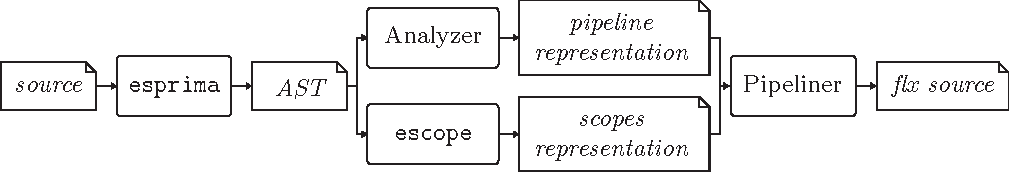
\includegraphics[width=\linewidth]{../resources/compiler-stream.pdf}
  \caption{Compilation chain}
  \label{fig:compilation}
\end{figure}

The chain of compilation is described in figure \ref{fig:compilation}.
The compiler extracts an AST from the source with \texttt{esprima}.
From this AST, the \textit{Analyzer} step identifies the limits of the different application parts and how they relate to form a pipeline.
This first step outputs a pipeline representation of the application.
Section \ref{chapter5:flx-compiler:analyzer} explains this first compilation step.
In the pipeline representation, the stages are not yet independent and encapsulated into fluxions.
From the AST, \texttt{escope} produces a representation of the memory scopes.
The \textit{Pipeliner} step analyzes the pipeline representation and the scopes representation to distribute the shared memory into independent groups of fluxions.
Section \ref{chapter5:flx-compiler:pipeliner} explains this second compilation step.

% \subsection{Analyzer step} \label{chapter5:flx-compiler:analyzer}

The limit between two application parts is defined by a rupture point.
The analyzer identifies these rupture points, and outputs a representation of the application in a pipeline form.
Application parts are the stages, and rupture points are the message streams of this pipeline.

\subsection{Rupture points} \label{chapter5:flx-compiler:analyzer:rupture}

A rupture point is a call of a loosely coupled function.
It is an asynchronous call without subsequent synchronization with the caller.
In \textit{Node.js}, I/O operations are asynchronous functions and indicate rupture points between two application parts.
Figure \ref{fig:basicrp} shows a code example of a rupture point with the illustration of the execution of the two application parts isolated into fluxions.
The two application parts are the caller of the asynchronous function call on one hand, and the callback provided to the asynchronous function call on the other hand.

\begin{figure}[h!]
  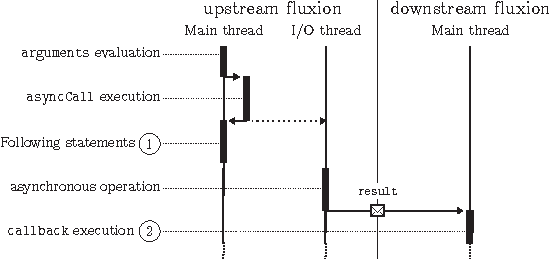
\includegraphics[width=\linewidth]{../resources/basicrp.pdf}
  \begin{code}
asyncCall(arguments, function callback(result){ //@\circled{2}@ });
// Following statements //@\circled{1}@
  \end{code}
  \caption{Rupture point interface}
  \label{fig:basicrp}
\end{figure}

A callback is a function passed as a parameter to a function call.
It is invoked by the callee to continue the execution with data not available in the caller context.
There are three kinds of callbacks, but only two are asynchronous: listeners and continuations.
The two corresponding types of rupture points are \textit{start} and \textit{post}.

\textbf{Start rupture points} (listeners) are on the border between the application and the outside, continuously receiving incoming user requests.
An example of a start rupture point is in listing \ref{lst:source}, between the call to \texttt{app.get()}, and its listener \texttt{handler}.
These rupture points indicate the input of a data stream in the program, and the beginning of a chain of fluxions to process this stream.

\textbf{Post rupture points} (continuations) represent a continuity in the execution flow after an asynchronous operation yielding a unique result, such as reading a file, or a database.
An example of a post rupture points is in listing \ref{lst:source}, between the call to \texttt{fs.readFile()}, and its continuation \texttt{reply}.

\subsection{Detection}

The compiler uses a list of common asynchronous callees, like the \texttt{express} and file system methods.
This list can be augmented to match asynchronous callees individually for any application.
To identify the callee, the analyzer walks the AST to find a call expression matching this list.

After the identification of the callee, the callback needs to be identified as well, to be encapsulated in the downstream fluxion.
For each asynchronous call detected, the compiler tests if one of the arguments is of type \texttt{function}.
Some callback functions are declared \textit{in situ}, and are trivially detected.
For variable identifiers, and other expressions, the analyzer tries to detect their type.
The analyzer walks back the AST to track their assignations and modifications, so as to determine their last value.





% \comment{TODO insert this}
% We developed the compiler core in node.js Javascript.
% There already exist sets of tools for manipulating code in Javascript.
% We used the Esprima suite of tools.